\chapter{Results}\label{chap:results}

\section{Controller Requirements}
\begin{itemize}
    \item It should be possible to select the area in which the bathymetric measurements are to be performed.
    \item The ASV should be able to autonomously plan and follow a route, such that the entire survey area is mapped.
    \item The controller should be robust to external disturbances.
    \item THU not exceed 30cm with a 95\% confidence interval.
\end{itemize}

Talk about the planing of the waypoints and the lines between them
\begin{figure}[H]
    \captionbox  
    {            
        Performance of the path following algorithm based on $\psi_\mathrm{ref}=\chi-\beta$ and using the LQR inner controller. The system is experiencing wind and wave disturbances, model perturbations and measurement noise.            
        \label{fig:path_lqr}                               
    }                                                                
    {                                                                 
        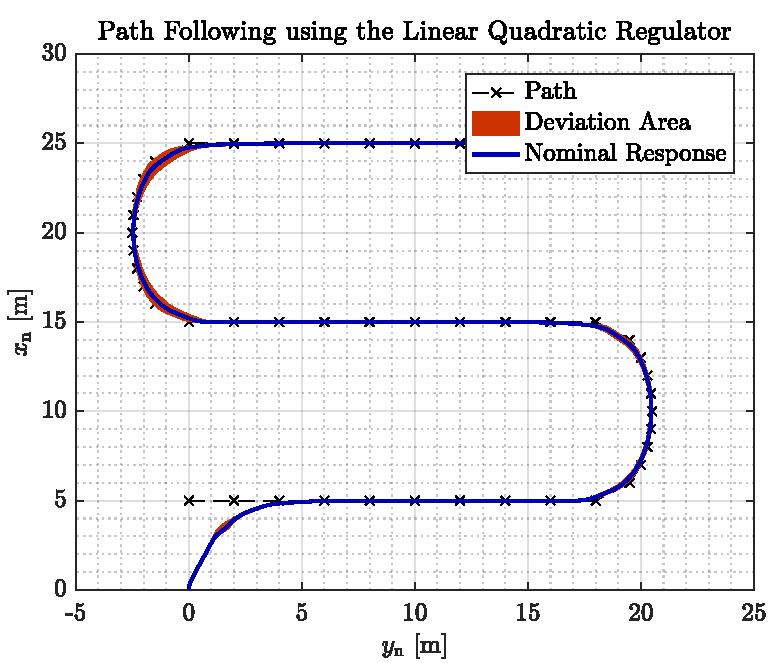
\includegraphics[width=.45\textwidth]{figures/path_lqr}         
    }                                                                  
    \hspace{5pt}                                                        
    \captionbox 
    {       
        Distance to the path when using the algorithm based on $\psi_\mathrm{ref}=\chi-\beta$ and the LQR inner controller .The system is experiencing wind and wave disturbances, model perturbations and measurement noise.                                                                  %\                         %\
        \label{fig:distlqr2}                                  
    }                                                                          
    {                                                                            
        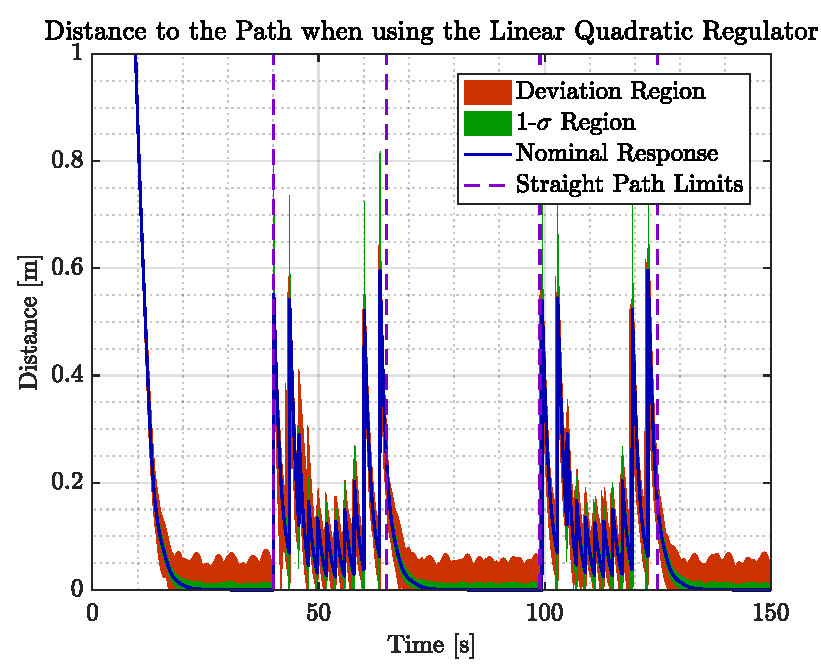
\includegraphics[width=.45\textwidth]{figures/dist_lqr}          
    }                                                                            
\end{figure}
\begin{figure}[H]
    \captionbox 
    {   
        Performance of the path following algorithm based on $\psi_\mathrm{ref}=\chi-\beta$ and using the $\mathcal{H}_\infty$ inner controller. The system is experiencing wind and wave disturbances, model perturbations and measurement noise. \label{fig:path_rob2}
    }                                                                 
    {                                                                  
        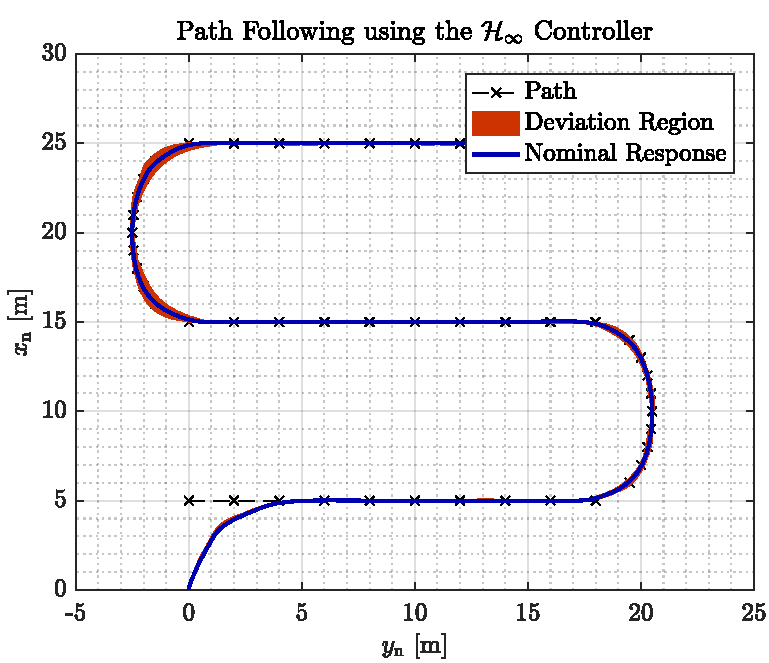
\includegraphics[width=.45\textwidth]{figures/path_rob}         
    }                                                                    
    \hspace{5pt}                                                          
    \captionbox  
    {      
        Distance to the path when using the algorithm based on $\psi_\mathrm{ref}=\chi-\beta$ and the $\mathcal{H}_\infty$ inner controller .The system is experiencing wind and wave disturbances, model perturbations and measurement noise.\label{fig:dist_rob2}
    }                                                                          
    {
        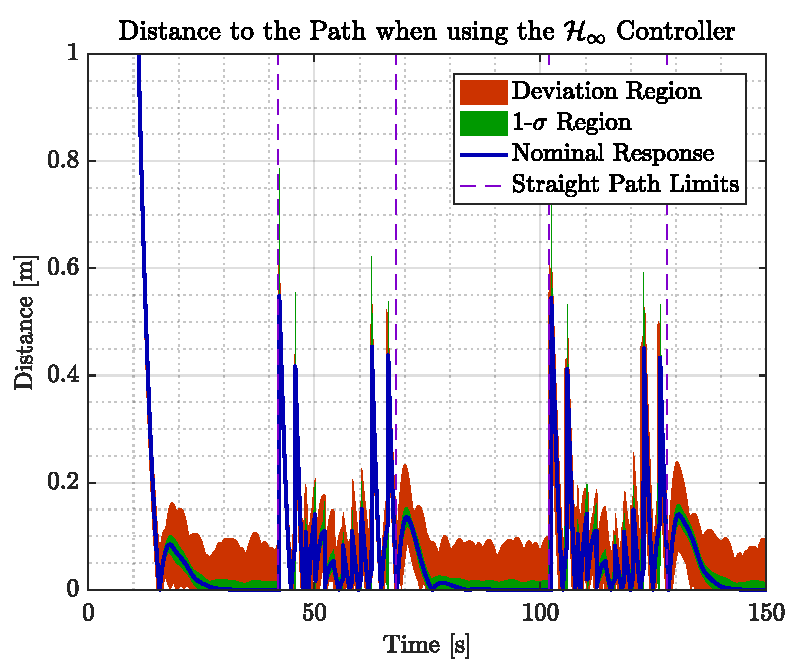
\includegraphics[width=.45\textwidth]{figures/dist_rob}
    }
\end{figure}



\section{Implementation Requirements}
\begin{itemize}
    \item The ASV should record and store data locally for extraction at the end of the survey.
    \item It should be possible to give the ASV a command to stop and steer it back to land.
\end{itemize}

We rosbag the files to save all the topics
Keyboard teleop node and VPN connection to run the nodes and stop them